\documentclass{standalone}
\usepackage{tikz}
\usepackage{ctex,siunitx}
\setCJKmainfont{Noto Serif CJK SC}
\usepackage{tkz-euclide}
\usepackage{amsmath}
\usepackage{wasysym}
\usetikzlibrary{patterns, calc}
\usetikzlibrary {decorations.pathmorphing, decorations.pathreplacing, decorations.shapes,}
\begin{document}
\small
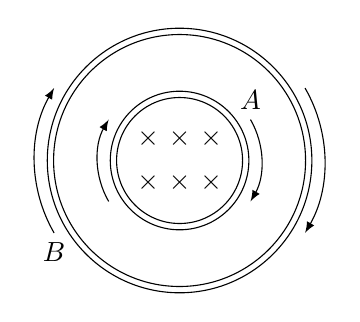
\begin{tikzpicture}[>=latex,scale=0.8]
  % \useasboundingbox(0.9,0)rectangle(5.1,5);
  \draw (0,0) circle (1);
  \draw (0,0) circle (1.1);
  \draw (0,0) circle (2);
  \draw (0,0) circle (2.1);
  \foreach \x in {-.5, 0, .5}
  \foreach \y in {-.35,.35}
  {
     \node at (\x,\y){$\times$};
  }
  
  \draw[->] (30:1.3) node [above]{$A$} arc (30:-30:1.3);
  \draw[->] (30:2.3) arc (30:-30:2.3);
  \draw[->] (210:1.3) arc (210:150:1.3);
  \draw[->] (210:2.3) node [below]{$B$} arc (210:150:2.3) ;
\end{tikzpicture}
\end{document}